\documentclass[11pt]{extarticle}
\usepackage[tmargin=1in,bmargin=1in,lmargin=1in,rmargin=1in]{geometry}
\usepackage[utf8]{inputenc}
\usepackage{tikz}
\usepackage{graphicx}
\usepackage{float}
\usepackage{setspace}
\usepackage{tabularx}
\usepackage[utf8]{inputenc}
\usepackage{caption}
\usepackage{subcaption}
\usepackage{framed}
\usepackage{enumitem}
\usepackage{amsmath}
\usepackage{mathpazo}
\usepackage{ragged2e}
\usepackage{titlesec}
\usepackage{framed}
\usepackage{color}   %May be necessary if you want to color links
\usepackage{hyperref}
\usepackage{footnotebackref}
\usepackage{listings}
\usepackage{xcolor}
\usepackage{fancyhdr}
\usepackage{lastpage}
\usepackage{pgfplots}
\usepackage{lscape}
\pgfplotsset{tick label style={font=\tiny}}

\hypersetup{
    colorlinks=true, %set true if you want colored links
    linktoc=section,     %set to all if you want both sections and subsections linked
    linkcolor=black,  %choose some color if you want links to stand out
}

\fancypagestyle{myheadings}
{
    \fancyhf{}
    \renewcommand{\footrulewidth}{0pt}
    \renewcommand{\headrulewidth}{0pt}
    \cfoot{Page \thepage\ of \pageref*{LastPage}}    
}

\fancypagestyle{plain}
{
    \fancyhf{}
    \chead{\small Delivery 03}
    \lhead{\small CS 353}
    \rhead{\small Spring 2022}
    % \renewcommand{\footrulewidth}{0.5pt}
    \renewcommand{\headrulewidth}{0.5pt}
    \cfoot{Page \thepage\ of \pageref*{LastPage}}    
}

\definecolor{mGreen}{rgb}{0,0.6,0}
\definecolor{mGray}{rgb}{0.5,0.5,0.5}
\definecolor{mPurple}{rgb}{0.58,0,0.82}
\definecolor{backgroundColour}{rgb}{0.95,0.95,0.92}

\lstdefinestyle{CStyle}{
    backgroundcolor=\color{backgroundColour},
    % backgroundcolor = \color{white},   
    commentstyle=\color{mGreen},
    keywordstyle=\color{magenta},
    numberstyle=\tiny\color{mGray},
    stringstyle=\color{mPurple},
    basicstyle=\footnotesize\bfseries\fontfamily{cmtt}\selectfont,
    breakatwhitespace=false,         
    breaklines=true,                 
    captionpos=b,                    
    keepspaces=true,                 
    numbers=left,                    
    numbersep=5pt,                  
    showspaces=false,                
    showstringspaces=false,
    showtabs=false,                  
    tabsize=2,
    frame = single,
    language=C
}

\title{\textbf{Project Delivery 03}}
\author{Aliza Rafique (05986); Asad Tariq (05439); Fahad Shaikh (05452); Faiz Haseeb (06224)}
\date{$8^{th}$ March 2022}


% Set formats for each heading level
\titleformat*{\section}{\Large\bfseries\fontfamily{phv}\selectfont}
\titleformat*{\subsection}{\large\bfseries\fontfamily{phv}\selectfont}
\titleformat*{\subsubsection}{\itshape\subsubsectionfont}

\providecommand\phantomsection{}

\doublespacing
\begin{document}
\begin{titlepage}
\thispagestyle{empty}
\begin{center}

\includegraphics[scale=0.40]{Figures/HU-LOGO--01.jpg}
\line(1,0){400}\\
[2mm]
\fontfamily{phv}\selectfont
\textbf{Project Proposal}\\
\line(2,0){250}\\
[0.5cm]
Submitted By\\
Aliza Rafique (05986)\\
Asad Tariq (05439)\\
Fahad Shaikh (05452)\\
%Nom 2 (NI 2) \\ %À enlever le commentaire si jamais vous êtes plusieurs
[1.5cm]
CS353\\
Software Engineering\\ 
[1.0cm]
Section\\
L1\\
[1.0cm]
Instructor\\
Mohsin Nagaria\\
[1.5cm]
From the department of Computer Science\\
Dhanani School of Science and Engineering\\
Habib University\\
3$^{rd}$ February, 2022
\end{center} 
\end{titlepage}
\newpage
\thispagestyle{empty}
\tableofcontents
\newpage
\pagestyle{plain}

\section{Non-Functional Requirements}
\justify
For our application, \textbf{Meri Raye}, we will have the following \textbf{non-functional requirements}:

\begin{enumerate}
    \item Performance:
                    \begin{enumerate}[label=(\alph*)]
                        \item The start-up time of the application should not be greater than approximately $10$ seconds.
                        \item The average response time of each feature of the application should also be approximately $10$ seconds (depending on which feature is being used).
                    \end{enumerate}
    \item Security:
                    \begin{enumerate}[label=(\alph*)]
                        \item The data in our database (MongoDB) should be secured with TLS/SSL encryption.
                        \item While logging in, the passwords in the password field of the login page should be hidden (most commonly achieved using asterisks).
                        \item After a certain number of incorrect attempts (5) to log in the application, the user's account will be locked for a short time period (5 minutes).
                    \end{enumerate}
    \item Reliability:
                    \begin{enumerate}[label=(\alph*)]
                        \item The application will need a stable internet connection (WiFi or 3g/4g) in order to view and post recommendations (which might or might not include pictures and videos).
                    \end{enumerate}
    \item Maintainability:
                    \begin{enumerate}
                        \item The development team will ensure software modularity and follow the principles of clean coding to make the software as maintainable as possible.
                    \end{enumerate}
    \item Accessibility:
                    \begin{enumerate}
                        \item Our application will be compatible with Android 7.0 and above so that it is accessible to as many users as possible including those who may not have access to newer smartphones.
                    \end{enumerate}
\end{enumerate}

\newpage
\justify
\section{Use-Case Diagram}
The \textbf{use-case} diagram of our application is as seen in \textbf{Figure} \ref{fig:use-case} below:
\begin{center}
    \begin{figure}[H]
        \centering
        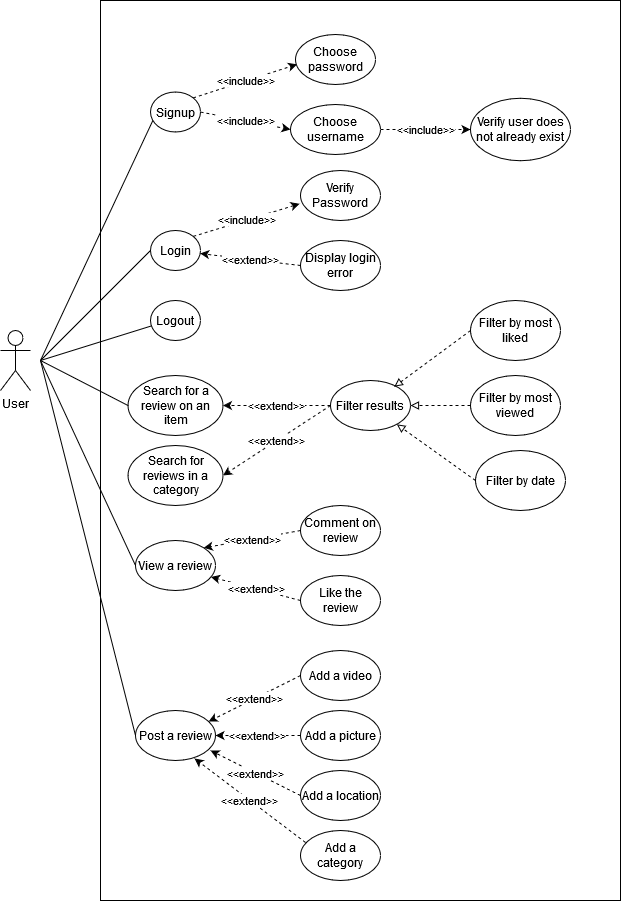
\includegraphics[width=4in]{Figures/Meri Raye Use Case.png}
        \caption{The use case diagram of the application.}
        \label{fig:use-case}
    \end{figure}
\end{center}

\newpage
\justify
\section{Use-Case Descriptions}
% Add use-case descriptions per the given template %

\subsection{Put name of the use-case here}
\begin{table}[H]
    \begin{center}
        \begin{tabular}{ |m{6cm}|p{6cm}| } 
           \hline
           \textbf{ID} &  [Unique ID of this use case]\\
           \hline
           \textbf{Title} &  [Enter the goal of the use case - preferably as a short, active verb phrase]\\
           \hline
           \textbf{Description} &  [Describe the goal and context of this use case. This is usually an expanded version of what you entered in the "Title" field.]\\
           \hline
           \textbf{Primary Actor} & [A person or a software/hardware system that interacts with your system to achieve the goal of this use case.] \\
           \hline
           \textbf{Preconditions} &  [Describe the state the system is in before the first event in this use case.]\\
           \hline
           \textbf{Postconditions} & [Describe the state the system is in after all the events in this use case have taken place.] \\
           \hline
           \textbf{Main Success Scenario} & [Describe the flow of events from preconditions to postconditions, when nothing goes wrong. This is the meat of the use case.]\\
           \hline
           \textbf{Extensions} &  [Describe all the other scenarios for this use case - including exceptions and error cases.]\\
           \hline
           \textbf{Status} &  [Development status]\\
           \hline
           \textbf{Priority} & [Priority of this use case] \\
           \hline
        \end{tabular}
    \end{center}
    \caption{\label{tab:Table 1} Detailed description for $<\textit{name-of-use-case}>$.}
\end{table}


\end{document}
